\section{Background}
\label{sec:background}

The methods presented in this paper were devised as part of the development of
a larger software toolbox for fully automatic analysis of very-high-resolution
SRµCT bone tomograms. Presently, the work is focused on the automatic analysis
of an experiment conducted to evaluate four different methodologies for
stimulating bone regeneration in goat mandibles, described below. The software
system is also being developed as preparatory work for the analysis of SRµCT
bone tomograms from 150 human patients in the MAXIBONE project
(\url{www.maxibone.eu}). This project aims to create personalized maxillary
bone regeneration by using culture-expanded autologous bone marrow stem cells
and biomaterials, for which clinical trials are presently being conducted. The
data set used in the present work is 35 high-resolution tomograms of old and
regenerated goat mandible bone samples, to evaluate the amount and health of
regenerated bone, and in particular, zooming in on osseointegration against the
titanium implants closer than was previously done.

\subsection{Background for the medical experiment} Installation of a dental
implant initiates the Regional Acceleratory Phenomenon (RAP), which implies an
acceleration of the different healing stages. RAP begins a few days after
implant installation, peaks at 1-2 months, and subsides after 6-24
months~\cite{frost1989}. In cortical bone, the non-vital mineralized tissue
initially needs to be resorbed prior to bone formation. In the cancellous
compartment, the implant installation mainly results in damage to marrow spaces
with resulting local bleeding and coagulum formation. The coagulum gradually
resorbs, collagen is laid down and replaced by osteoid, and eventually --- if
sufficient blood supply is present --- woven immature bone develops, and
sequentially osseointegration is initiated~\cite{frost1989}. After 6-12 weeks
of healing, most of the woven bone is mineralized and bone marrow containing
blood vessels, adipocytes, and mesenchymal cells can be observed surrounding
the trabeculae in the mineralized bone~\cite{Berglundh2003, Abrahamsson2004}. A
cement line, thickness of 0.2-5µm, will be deposited directly on the implant
surface during continuous bone formation. The biological fixation of the
implant initiates only a few days after implant installation, where the
osteoblasts begin to deposit collagen matrix on the cement line. This early
deposition of calcified matrix followed by the arrangement of woven bone and
later mature cancellous bone develops in a 3D manner delimiting the marrow
space~\cite{Franchi2004}.

\subsection{Physical samples}

The experiment evaluated four methods for stimulating maxillary bone
regeneration. 5 critical size defects were introduced to 7 goats. Four defects
were used to asses bone regeneration methods, and one was a control sample.
Peri-implant vertical bone augmentation was performed using autologous bone and
two different calcium phosphate bone substitutes. The bone specimens were
evaluated undecalcified. The specimen preparation was performed at the
Department of Biomaterials at Gothenburg University, Sweden. The specimens were
initially fixated in 4\% paraformaldehyde. Dehydration of the specimens was
performed in increasing concentrations of ethanol to eliminate fat and water
content. Furthermore, specimens were infiltrated with methylmethacrylate (MMA)
and embedded in molds 12 mm in diameter and 20 mm in
height~\cite{NELDAM2015682}. They were scanned at the European Synchrotron
Radiation Facility (ESRF) in Grenoble, France. The advantage of using MMA is
greater tissue penetration than water-soluble methacrylates. This is an
advantage when preparing larger specimens such as bone biopsies containing
dental implants. Furthermore, the histological quality of bone sections is
generally higher for MMA-embedded specimens compared to water-soluble
methacrylates~\cite{erben1997}. Additionally, tissue shrinkage is less than 2\%
when using MMA-embedded bone and cartilage specimens~\cite{ferguson1999}.

Physical samples were prepared for SRµCT scanning by cutting out portions from
the larger cylindrical biopsies. Within these samples, we find the titanium
dental implant (Astra Tech OsseoSpeed, ST Molndal, Sweden).  It is 3.5mm in
diameter and 8mm long. Along its length, the lower 5.5mm has larger threads and
is attached to the recipient bone. The upper 2.5mm has smaller threads and is
where the newly formed bone is to be assessed. Surrounding the bone and implant
contact region are cavities containing resin, air, blood vessels and other
fibrous tissue.

\begin{figure}
  \centering
  \begin{tabular}{cc}
    (a) & \begin{tabular}{c} 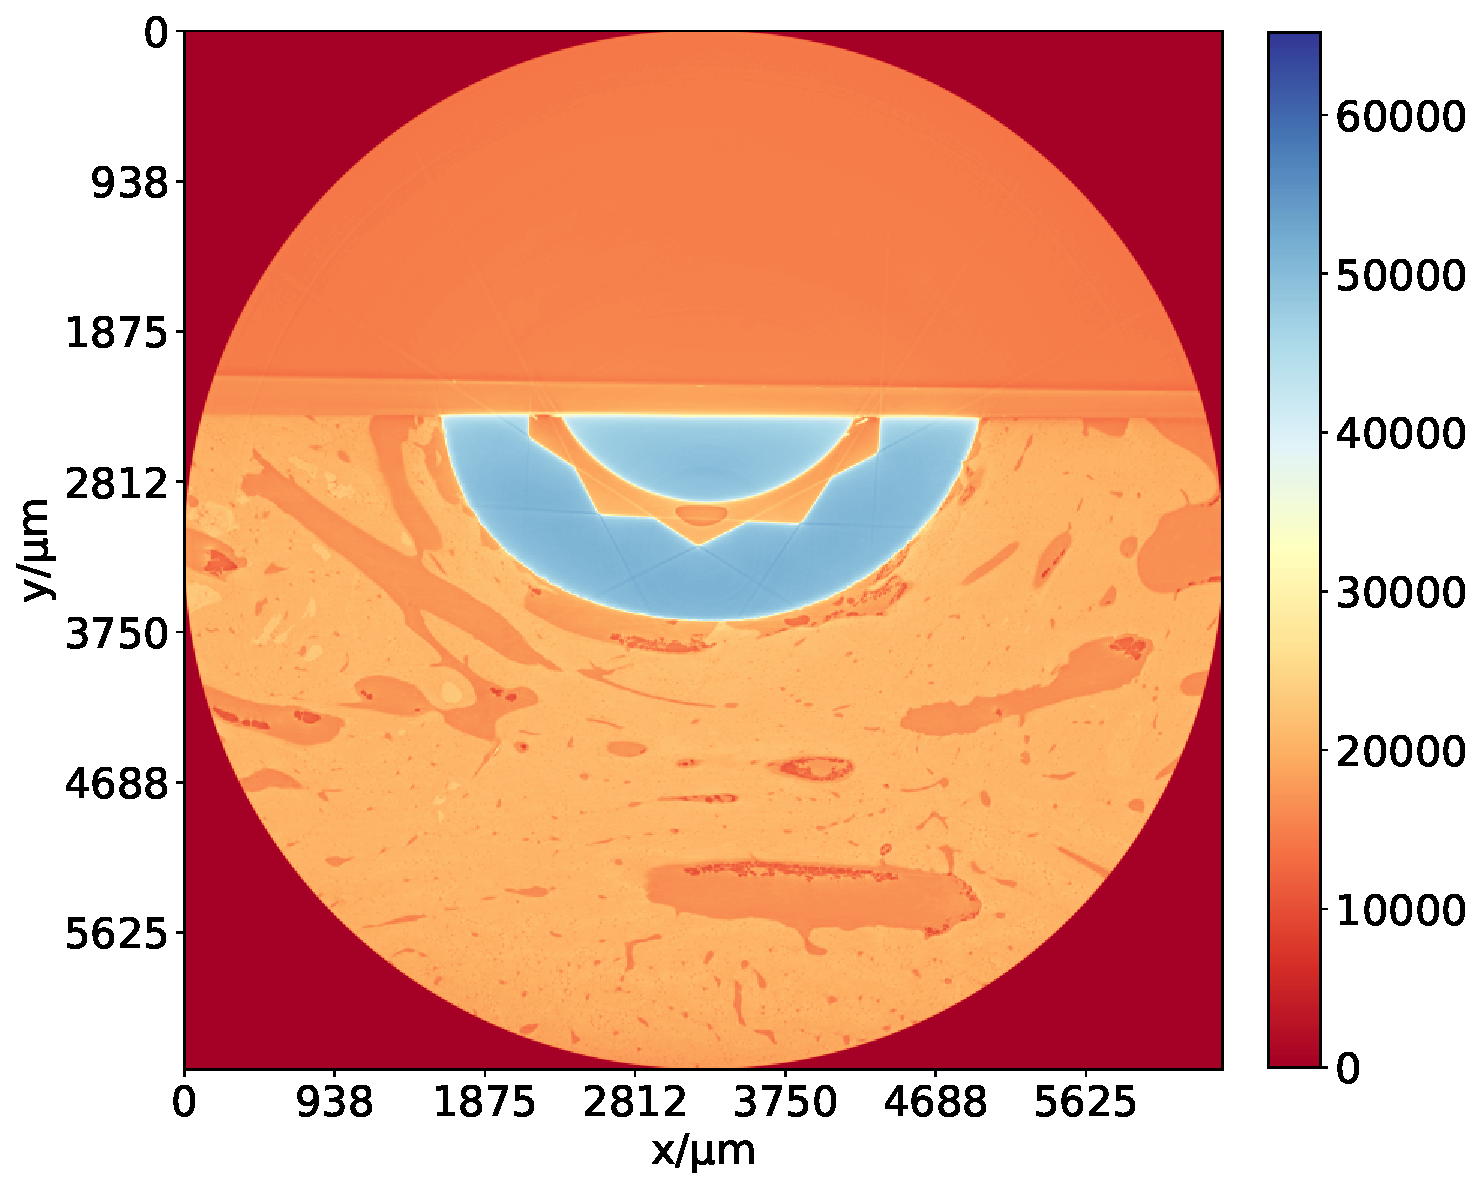
\includegraphics[width=0.81\linewidth]{generated/770c_pag_full_yx.pdf}\end{tabular}\\
    (b) & \begin{tabular}{c} 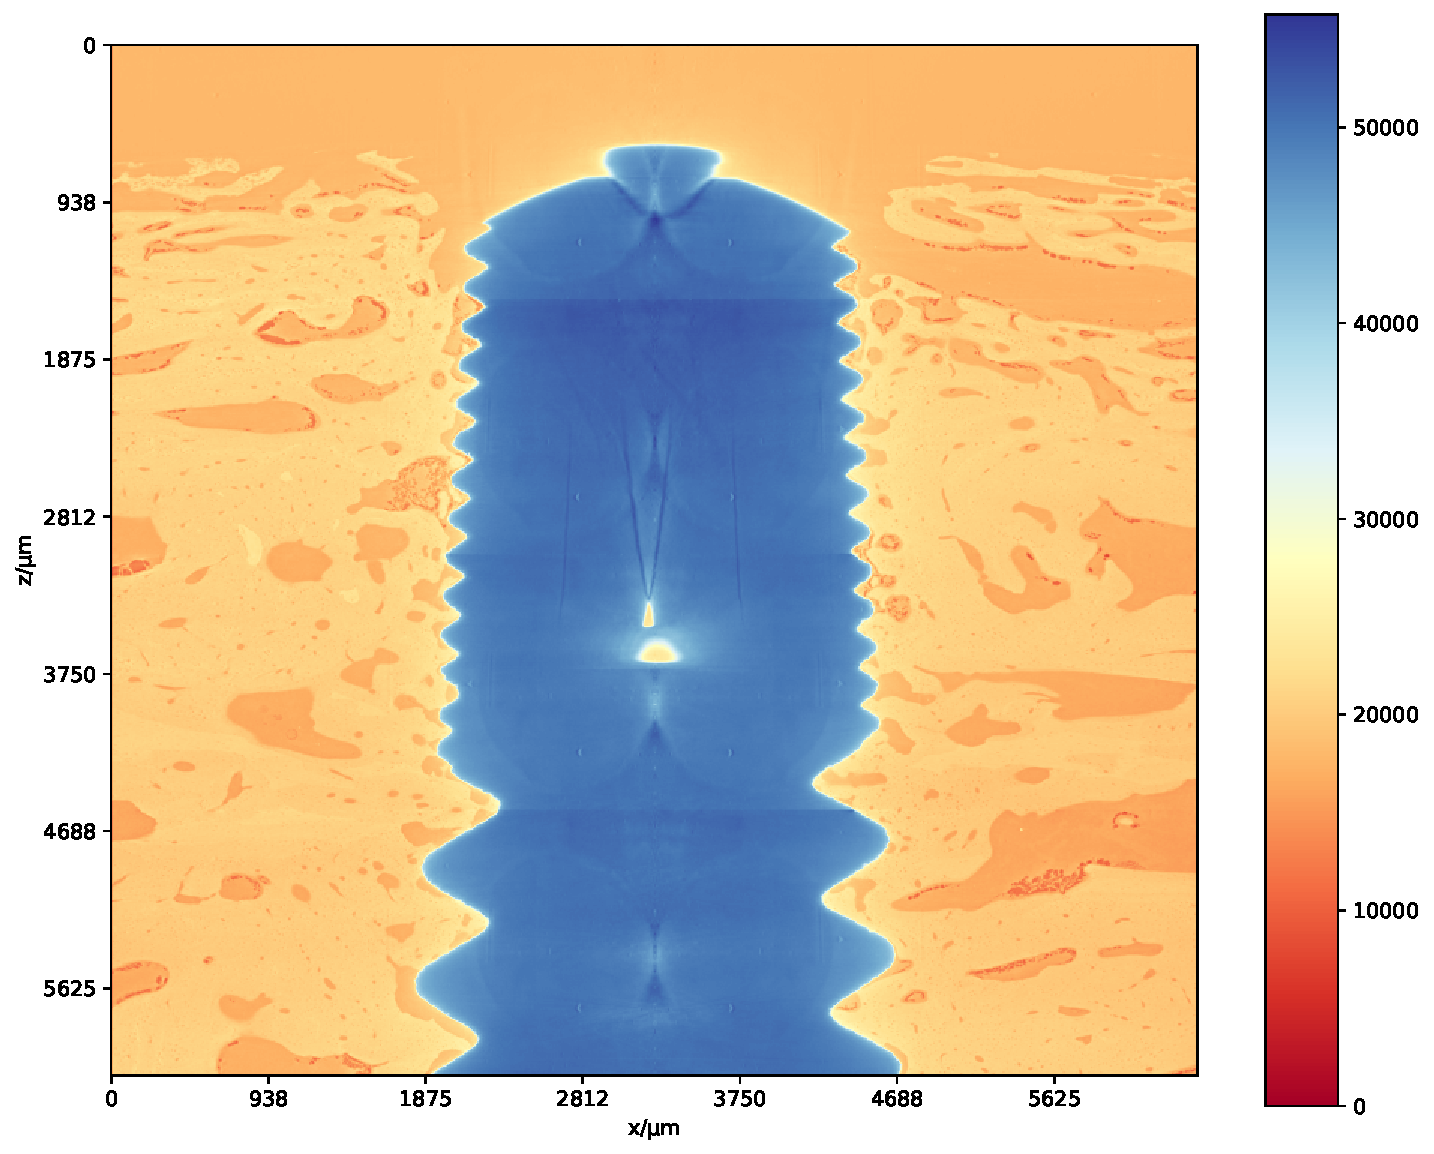
\includegraphics[width=0.81\linewidth]{generated/770c_pag_full_zx.pdf}\end{tabular}\\
    (c) & \begin{tabular}{c} 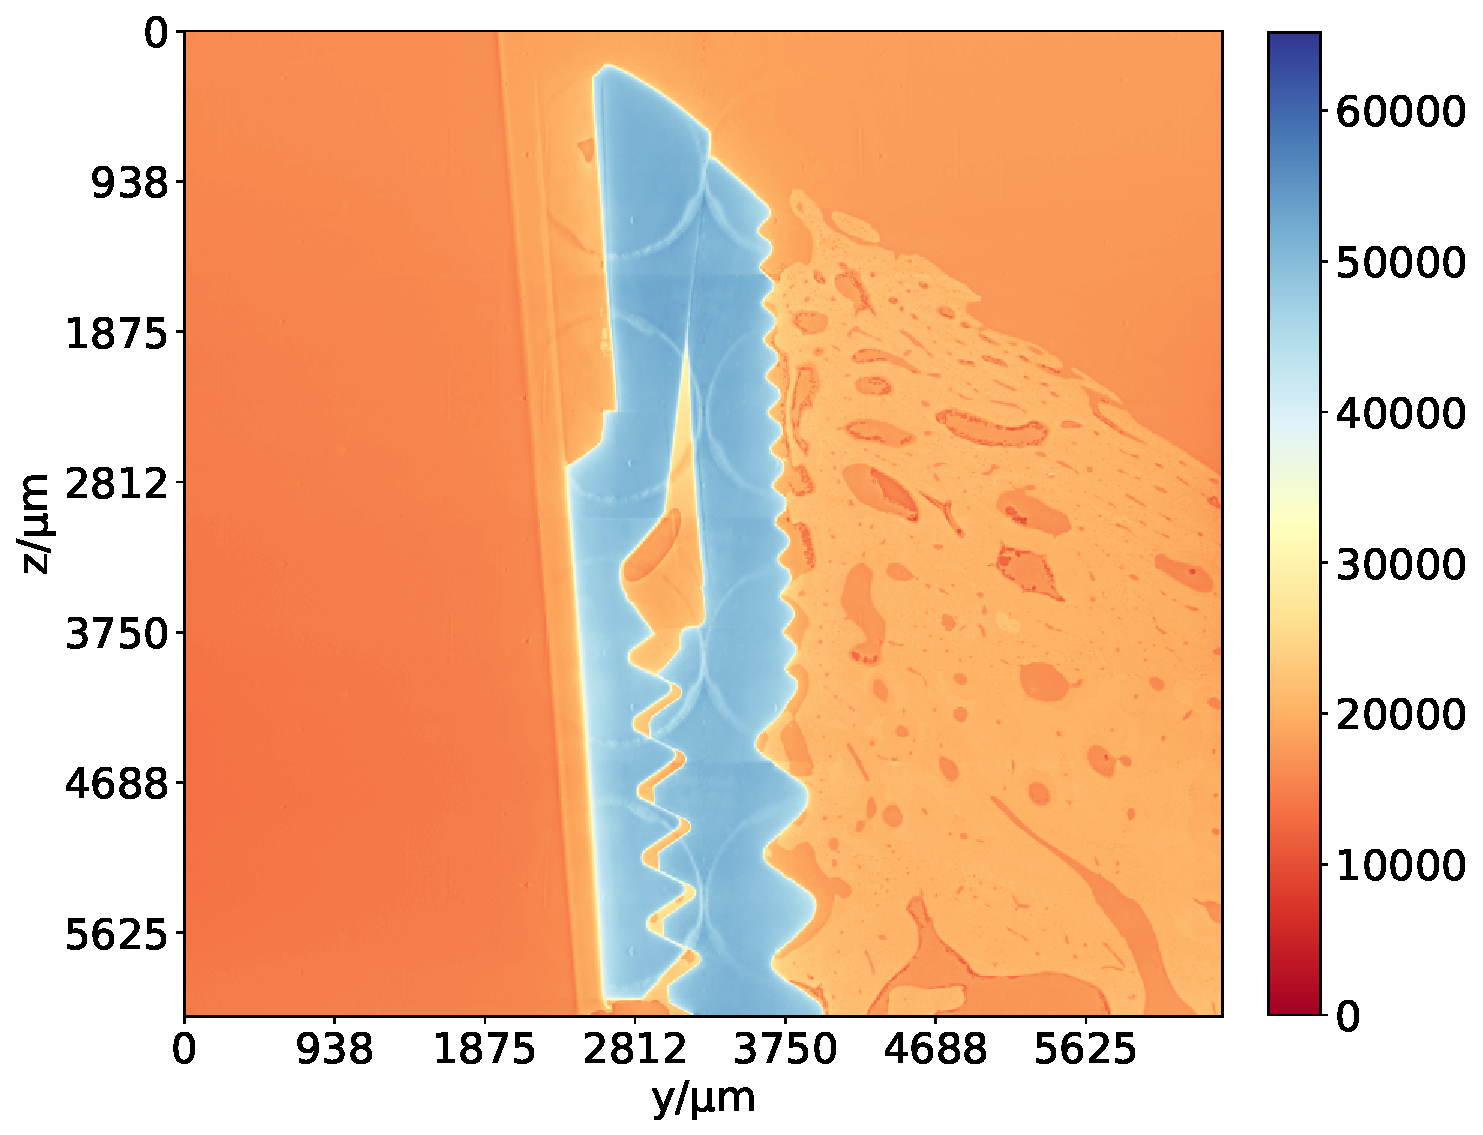
\includegraphics[width=0.81\linewidth]{generated/770c_pag_full_zy.pdf}\end{tabular}
  \end{tabular}
  \caption{
    Cross sections of a sample in YX-, ZX- and ZY-planes respectively. A voxel
    has a size of 1.875µm.
  }
\label{fig:3viewsample}
\end{figure}

% TODO: description of color depends on final colormap -- still better than lighter/dark
A cut sample is shown in three different cross-sectional views in
\Cref{fig:3viewsample}. Each material has a unique density and thus absorption.
The titanium implant shown in blue has a higher absorption level than bone.
Bone material shown in light orange has higher absorption than its surrounding
dark orange-colored regions containing blood vessel tissue, air and resin.

\subsubsection{Data acquisition}

It can be difficult to study and evaluate the bone structure and blood network
without destroying or manipulating the sample. X-ray computed tomography is a
widely used tool for non-intrusive medical imaging. By exposing a subject to
X-rays, we can map the linear attenuation coefficient of the passing rays. Each
ray is attenuated relatively to the density and composition of the material it
passes. By rotating either the scanner or the sample we can get a full 3D image
representation of the inner structure of the sample. Each volumetric pixel
(voxel) then represents the X-ray attenuation at its spatial position. In this
way, X-rays can reliably be used to internally characterize samples in a
non-intrusive and non-destructive manner. Medical CT scans can provide spatial
resolutions on the order of submillimetre scale \citep{medicalct}. The more
modern micro-computed tomography (µCT) can provide much higher spatial
resolution on the micrometer scale \citep{srexptime}.

This work focuses on a data set acquired by Synchrotron Radiation micro-CT
(SRµCT). For this imaging technique, electrons are accelerated to
ultra-relativistic speeds in trajectories directed by strong magnetic fields.
The resulting X-ray beam provides a high photon flux allowing for very short
exposure times \citep{srexptime}. This can help counter Poisson noise from
suboptimal photon count \citep{srnoise}. Contrary to both CT and µCT, this
approach requires a large particle accelerator and is not standard medical or
laboratory equipment. However, SRµCT offers an even better spatial resolution
of up to 0.1 µm, and much higher image quality due to fewer distortive X-ray
effects. The resulting beams are high in brilliance and collimation, which
gives a very clear signal. Artifacts from beam-hardening are minimized due to
synchrotron radiation X-rays being characterized by their practically
mono-energetic spectrum.

The tomograms presented here have been acquired at the ID19 beamline at the
European Synchrotron Radiation Facility (ESRF) in Grenoble, France. They were
reconstructed\citep{sporring} at the ID19 beamline. A standard filtered
back-projection algorithm was applied via the ESRF in-house developed software
PyHST~\citep{NELDAM2015682,pyhst}. PyHST was applied to improve reconstruction
quality, hence reducing ring artifacts, and to reduce the required data volume
if necessary~\cite{MIRONE201441}. The tomograms were acquired at 50 keV.

The physical field of view of a single image sample is about 6.5mm in each
direction. Each sample contains voxels with a spatial resolution of 1.875µm.
The samples are scanned in chunks of 4-6 sub-volumes through the height of the
implant, depending on the initial size of a sample.

%%% Local Variables:
%%% mode: latex
%%% TeX-master: "main"
%%% End:
